Find the best fit parabola for these 4 data points. Recall that a parabola can be defined using the explicit function $y=ax^2+bx+c$.

\begin{align*}
    (0, 1), (1, 0), (3, 2), (5, 4)
\end{align*}

\begin{solution}\
\begin{lstlisting}
hold on
x_data = [0; 1; 3; 5];
y_data = [1; 0; 2; 4];
plot(x_data, y_data, '*')
A_data = [x_data.^2 x_data ones(size(x_data))];
p = A_data\y_data
\end{lstlisting}

\begin{align*}
    p = \begin{bmatrix}
        0.1910 \\ -0.2663 \\ 0.6784
    \end{bmatrix} \\
    y = 0.1910 x^2 - 0.2663x + 0.6784
\end{align*}

\begin{lstlisting}
x = linspace(-1, 6, 1000)';
A = [x.^2 x ones(size(x))];
y = A * p;
plot(x, y)
\end{lstlisting}

\begin{center}
    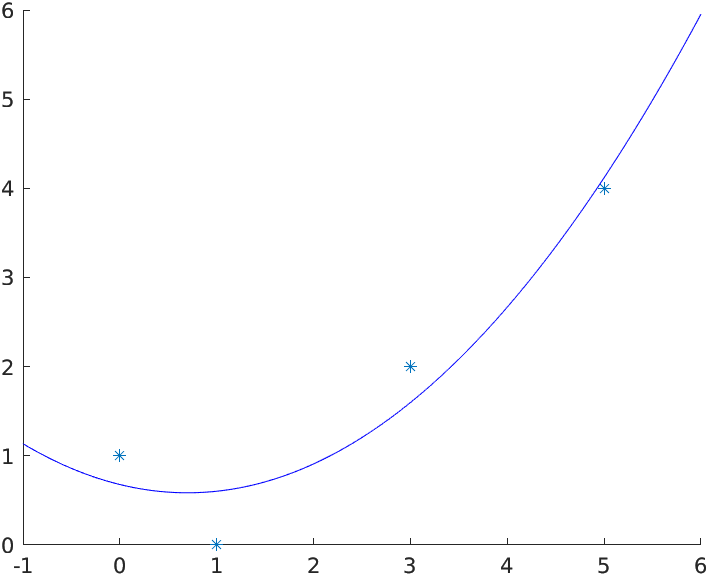
\includegraphics[width=0.5\textwidth]{img/e12p1.png}
\end{center}
\end{solution}